\section{基于二分类机器学习}
二分类机器学习的算法有很多,常见的有逻辑回归logical regression(lg)和支持向量机svm。本次课题选择这两种分类模型探究识别恶意URL的课题。基于二分类机器学习恶意URL检测算法如下:
\begin{algorithm}[!h]
    \SetAlgoNoLine
    % \SetAlgoNoLine可以去掉竖线
    \caption{基于二分类机器学习恶意URL检测算法}
    \KwIn{URL Text}
    \KwOut{The Evaluate and Prediction Outputs}
    initialization\;
    load data\; 
    spilt URL text into words\;
    vectorize the words to get the feature matrix\;
    split the data into training set and validating set\;
    \eIf{logical regression}{
            use LogisticRegression classifier\;
        }{
            use SVM classifier\;
        }
    train training set\;
    validate and evaluate the prediction\;
\end{algorithm}
\subsection{模型算法原理}
\subsubsection{Logistic Regression逻辑回归}
逻辑回归是这样的一个过程:面对一个回归或者分类问题,建立代价函数,然后通过优化方法迭代求解出最优的模型参数,然后测试验证我们这个求解的模型的好坏。
\\\indent{}逻辑回归虽然名字里带“回归”,但是它实际上是一种分类方法,主要用于两分类问题(即输出只有两种,分别代表两个类别)。回归模型中,y是一个定性变量,比如y=0或1,逻辑回归方法主要应用于研究某些事件发生的概率。
\\\indent{}常规步骤如下:
\begin{itemize}
    \item 寻找$h$函数(即预测函数)
    \item 构造$J$函数(损失函数)
    \item 想办法使得$J$函数最小并求得回归参数($\theta$)
\end{itemize}
\subsubsection{SVm支持向量机}
分类作为数据挖掘领域中一项非常重要的任务,它的目的是学会一个分类函数或分类模型(或者叫做分类器),而支持向量机本身便是一种监督式学习的方法,,它广泛的应用于统计分类以及回归分析中。支持向量机(SVM)是90年代中期发展起来的基于统计学习理论的一种机器学习方法,通过寻求结构化风险最小来提高学习机泛化能力,实现经验风险和置信范围的最小化,从而达到在统计样本量较少的情况下,亦能获得良好统计规律的目的。
通俗来讲,它是一种二类分类模型,其基本模型定义为特征空间上的间隔最大的线性分类器,即支持向量机的学习策略便是间隔最大化,最终可转化为一个凸二次规划问题的求解。
SVM作为传统机器学习的一个非常重要的分类算法,它是一种通用的前馈网络类型,最早是由Vladimir N.Vapnik 和 Alexey Ya.Chervonenkis在1963年[p]提出,目前的版本(soft margin)是Corinna Cortes 和 Vapnik在1993年提出,1995年[p]发表。深度学习(2012)出现之前,SVM被认为是机器学习中近十几年最成功表现最好的算法。
\subsection{数据向量化}
无论是恶意请求数据集还是正常请求数据集,都是不定长的字符串列表,很难直接用逻辑回归算法对这些不规律的数据进行处理,所以,需要找到这些文本的数字特征,用来训练我们的检测模型。
\\\indent{}在这里,我们使用 TD-IDF 来作为文本的特征,并以数字矩阵的形式进行输出。TD-IDF 是一种用于资讯检索与文本挖掘的常用加权技术,被经常用于描述文本特征。TF表示词条在某文档中出现的频率。IDF表示的是如果包含词条的文档越少,则IDF越大,说明该词条具有很好的类别区分能力。TF-IDF倾向于过滤掉常见的词语,保留重要的词语。
\\\indent{}TD-IDF输入的是文本的词语,所我们需要将url分词。我们选择通过长度为N的滑动窗口将文本分割为N-Gram序列。n越大,产生的字母组合种类越多,产生的向量维度会更大,运算开销会增大,考虑到服务器的性能,这里我们选择n=2。
\\\indent{}经过分词,再TD-IDF处理,我们得到url的特征矩阵。输出格式如下(表\ref{fig:vec}):
\begin{figure}[!h]
    \setlength{\abovecaptionskip}{0.cm}
    \setlength{\belowcaptionskip}{-0.cm}
    \centering
     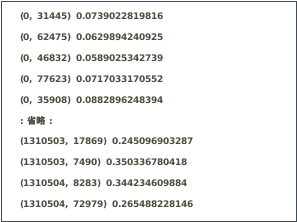
\includegraphics[scale=0.55]{Figs/vec.png}
    \caption{URL向量化后的部分样例}
    \label{fig:vec}
\end{figure}
\\\indent{}可以看出特征矩阵的元素由[(i,j) weight]三个元素组成,矩阵元素[(i,j) weight] 表示编号为j的词片在编号为i的URL下的 TD-IDF值(weight)。
\subsection{训练模型}
得到了url的特征矩阵后,我们需要将数据集分为训练集和测试集。训练集用于训练模型,测试集则是根据训练集的训练结果来评判最终的训练效果。这里我们训练集占了所有数据集合的$80\%$,测试集是$20\%$。
\subsection{测试模型}
经过训练之后使用classifier的score选择一批测试数据来计算模型的准确度,测试数据(x\_test,y\_test)我们已经在上一步中分割得到。
\subsection{实验结果对比}
实验训练均采用默认数据集:
\begin{itemize}
    \item goodfile='good2.txt'
    \item badfile='bad\_waf.txt'
    \item testfile='good1.txt'
\end{itemize}
\ \ \ \ 采用lg和SVM方法得到的训练集正确率和测试集正确率如下(表 \ref{table:no_keams})
\begin{table}[!ht]
    \setlength{\abovecaptionskip}{0.cm}
    \setlength{\belowcaptionskip}{-0.cm}
    \caption{lg和svm分类器训练结果}
    \centering
    \label{table:no_keams}    
    \begin{tabular}{|c|c|c|}
        \hline
        &LG&SVM\\
        \hline
        Training Accuracy&0.9987&0.9632\\
        \hline
        Testing Accuracy&0.9974&0.8013\\
        \hline
    \end{tabular}
\end{table}
\subsection{模型结构改进}
可见lg分类模型对URL的识别相比svm更加精确,整体样本是70052个,误差上多了2486个,而且训练时间也长于lg分类器。
\\\indent{}对于这种情况,经过分析和查阅资料后发现,svm对数据的异常点(离群值)比较敏感,因为其训练只需要支持向量,有效样本本来就不高,一旦被干扰,预测结果难以预料。同时一般输入svm的数据维度不宜太高,而本文训练的数据集有4117维,所以决定在处理前加入降维模块。 
\\\indent{}本文选择用kmeans降维。该算法的主要思想是通过迭代过程把数据集划分为不同的类别,使得评价聚类性能的准则函数达到最优,从而使生成的每个聚类内部紧凑,类间独立。 
\\\indent{}(表 \ref{table:svm_use})是对于svm选择80维和150维聚类,加入降维后的结果: 
\begin{table}[!ht]
    \setlength{\abovecaptionskip}{0.cm}
    \setlength{\belowcaptionskip}{-0.cm}
    \caption{svm分类器加入Kmeans降维训练后结果}
    \centering
    \label{table:svm_use}    
    \begin{tabular}{|c|c|c|}
        \hline
        &80维&150维\\
        \hline
        Training Accuracy&0.9931&0.9913\\
        \hline
        Testing Accuracy&0.9847&0.9854\\
        \hline
    \end{tabular}
\end{table}
\\\indent{}可见,对数据降维后svm运行的速度和正确率都大大提升了,说明加入降维之后是有效果的。
\\\indent{}那么对于lg分类器来说,是不是加入聚类之后效果也有提升呢?根据(表 \ref{table:lg_use})来看,结果没有太大变化,甚至相对于原来的正确率有所下降,可见不同模型有不同的模型优化方法,算法的使用场景不是完全相同的。
\begin{table}[!ht]
    \setlength{\abovecaptionskip}{0.cm}
    \setlength{\belowcaptionskip}{-0.cm}
    \caption{lg分类器加入Kmeans降维训练后结果}
    \centering
    \label{table:lg_use}    
    \begin{tabular}{|c|c|c|}
        \hline
        &80维&150维\\
        \hline
        Training Accuracy&0.9963&0.9979\\
        \hline
        Testing Accuracy&0.9949&0.9943\\
        \hline
    \end{tabular}
\end{table}